\documentclass{article}

\usepackage{phdstyle}
\usepackage[numbers]{natbib}

\begin{document}
\tableofcontents
\newpage

\section{Spin decoherence in a perfectly aligned ring}
Spin coherence refers to a measure or quality of preservation of polarization in an initially fully polarized beam.~\citep[p.~205]{Eremey:Thesis}

When a polarized beam is injected into a storage ring, the spins of the beam particles start precessing around the vertical (guiding) magnetic field. The precession frequency is dependent upon the equilibrium-level energy of the particle, which differs for the particles in the beam.

This does not pose a problem when the initial polarization is vertical; however, the FS storage ring method requires spin polarization along the momentum vector, i.e., in the horizontal plane. Therefore, spin decoherence is an inherent weakness of the FS method.

\subsection{Spin coherence time requirements}
The spin coherence time (SCT) for an FS method performed in a perfectly aligned storage ring is determined by the smallest detectable angle by which the beam polarization vector is tilted from the horizontal plane by EDM alone. For the sensitivity level of $10^{-29}~e\cdot cm$ it is about $5\cdot10^{-6}$.~\cite{BNL:Deuteron2008}

According to the T-BMT equation,
\[
\W_{EDM,x} = \eta\frac{qE_x}{2mc},
\]
where $\eta$ is the proportionality factor between the EDM and spin, equaling $10^{-15}$ for the deuteron, for the given EDM sensitivity limit.~\citep[p.~206]{Eremey:Thesis}

For the deuteron BNL FS storage ring, $E_x = 12$ MV/m,~\citep[p.~19]{BNL:Deuteron2008} and so $\W_{EDM,x}\approx 10^{-9}$ rad/sec. This gives an SCT of approximately 1000 seconds in order that the vertical polarization reaches a detectable level of 1$\mu$rad.~\citep[p.~207]{Eremey:Thesis}

\subsection{Origin of decoherence}\label{sec:Decoh_origin}
Spin decoherence in a particle bunch is caused by the difference in the spin precession angular velocities, which, in turn, is due to the difference in the particles' orbit lengths and momentum values. This can be seen from the following considerations.

When a particle with spin enters a magnetic field area, the spin vector starts turning about the magnetic field vector with an angular velocity defined by the T-BMT equation~\eqref{eq:TBMT_MDM}:
\begin{equation*}
  \vec\W_{MDM} = \frac qm G\vec B.
\end{equation*}
Upon exiting the field area, the spin has turned by an angle
\begin{equation*}
  \theta = \Delta t\cdot\W_{MDM} = \frac Lv \cdot \frac qm GB\cdot \frac{\gamma_0}{\gamma_0} = \frac{L\gamma_0 GB}{B\rho} = \frac L\rho\gamma_0\cdot G,
\end{equation*}
where $L$ is the path length inside the B-field, and $B\rho = p/q$ is the magnetic rigidity.

In the simple model considered so far, the influence of the orbital dynamics upon the spin dynamics is expressed by the $\gamma_0 L/\rho$ (effective gamma) term. In the case of the reference particle, $\gamma_0L/\rho = \gamma_0$, while for a particle involved in betatron motion, the effective gamma is different from $\gamma_0$. In the following sections we will specify the connection between the spin and orbital dynamics of a particle further in a more general fashion.

\subsubsection{Equilibrium momentum shift}
The longitudinal dynamics of a charged particle on the reference orbit in a storage ring is described by the system of equations:
\begin{equation*}
  \begin{cases}
    \ddt{\varphi} &= -\w_{RF}\eta\delta, \\
    \ddt{\delta} &= \frac{q V_{RF}\w_{RF}}{2\pi h\beta^2E}\sin\varphi.
  \end{cases}
\end{equation*}
In the equations above: $\varphi$ is the phase deviation from the reference $\varphi_0 = 0$; $\delta = \frac{\Delta p}{p_0}$ is the relative momentum deviation from the momentum $p_0$ of the reference particle; $V_{RF}$, $\w_{RF}$ are the voltage and oscilation frequency of the RF field; $\eta = \alpha_0 - \gamma^{-2}$ is the slip factor, with $\alpha_0$ being the compaction factor defined by $\sfrac{\Delta L}{L} = \alpha_0\delta$, and $L$ being the orbit length; $h$ is the harmonic number; $E$ is the total energy of the accelerated particle. $\w_{RF} = 2\pi h f_{rev}$, where $f_{rev}=T_{rev}^{-1}$ is the beam revolution frequency.

The solutions of this system form a family of ellipses in the $(\varphi, \delta)$ space, centered at $(0,0)$. However, if we consider a particle involved in betatron oscillations, and use a higher-order Taylor expansion of the compaction factor $\alpha = \alpha_0 + \alpha_1\delta$, the first equation of the system transforms into:~\citep[p.~2579]{Senichev:IPAC13}
\[
\ddt{\varphi} = -\w_{RF} \bkt*{\bkt{\frac{\Delta L}{L}}_\beta + \bkt{\alpha_0 + \gamma^{-2}}\delta + \bkt{\alpha_1 - \alpha_0\gamma^{-2} + \gamma^{-4}}\delta^2},
\]
where $\bkt{\frac{\Delta L}{L}}_\beta = \frac{\pi}{2L}\bkt*{\varepsilon_xQ_x + \varepsilon_yQ_y},$ is the betatron motion-related orbit lengthening; $\varepsilon_x$ and $\varepsilon_y$ are the horizontal and vertical beam emittances, and $Q_x$ and $Q_y$ are the horizontal and vertical tunes.~\citep[p.~2580]{Senichev:IPAC13}

The solutions of the modified system are no longer centered at the same point. Orbit-lengthening and momentum deviation cause an equilibrium-level momentum momentum shift~\citep[p.~2581]{Senichev:IPAC13}
\begin{equation}\label{eq:EquLevMom_shift}
  \Delta\delta_{eq} = \frac{\gamma_0^2}{\gamma_0^2\alpha_0 - 1}\bkt*{\frac{\delta_m^2}{2}\bkt{\alpha_1 - \alpha_0\gamma^{-2} + \gamma_0^{-4}} + \bkt{\frac{\Delta L}{L}}_\beta},
\end{equation}
where $\delta_m$ is the amplitude of synchrotron oscillations.

%% The equilibrium energy spread, associated with this momentum shift, of the beam particles results in a spin tune spread~\citep[p.~2581]{Senichev:IPAC13}

\subsubsection{Effective Lorentz factor}
The equilibrium energy associated with the momentum shift~\eqref{eq:EquLevMom_shift}, termed the \emph{effective Lorentz factor}, is~\cite{Senichev:FDM}
\begin{equation}\label{eq:EffectiveGamma}
  \gamma_{eff} = \gamma_0 + \beta_0^2\gamma_0\cdot\Delta\delta_{eq},
\end{equation}
where $\gamma_0$, $\beta_0$ are the reference particle's Lorentz factor and normalized speed. Equations~\eqref{eq:EquLevMom_shift} and~\eqref{eq:EffectiveGamma} define the link between the particle spin and orbital dynamics.

\subsection{Sextupoles for the reduction of decoherence}\label{sec:Sextupole_decoherence_suppression}
To minimize the spin decoherence dur to betatron motion and momentum deviation, sextupoles (or octupoles) may be used~\citep[p.~212]{Eremey:Thesis}

A sextupole of strength
\[
S_{sext} = \frac{1}{B\rho} \pddx{B_y}[x][2],
\]
where $B\rho$ is the magnetic rigidity, affects the first-order compaction factor as~\citep[p.~2581]{Senichev:IPAC13}
\begin{align}
  \Delta \alpha_{1,sext} &= -\frac{S_{sext}D_0^3}{L}, \label{eq:Sext_compaction_effect}
  \intertext{and simultaneously the orbit length as}
  \bkt{\frac{\Delta L}{L}}_{sext} &= \mp \frac{S_{sext}D_0\beta_{x,y}W_{x,y}}{L}, \label{eq:Sext_OL_effect}
\end{align}
where $D(s,\delta) = D_0(s) + D_1(s)\delta$ is the dispersion.

In the following sections, we will call the decoherence accociated with horizontal/vertical betatron, and synchrotron oscillations, respectively X-/Y-, and D-decoherence. 

It can be observed from eqs~\cref{eq:Sext_compaction_effect,eq:Sext_OL_effect}, that three sextupole families are required for the reduction of decoherence, placed in the maxima of: $\beta_x$, $beta_y$ for the reduction of X-,Y-decoherence, and $D_0$ for D-decoherence.

\subsubsection{Simulation}
In order to check the effectiveness of the sextupole method for the suppression of decoherence, a simulation was carried out using the COSY INFINITY code.

We took a perfectly aligned FS lattice, with three families of sextupoles (SX, SY, SD) placed as was explained at the end of section~\ref{sec:Sextupole_decoherence_suppression}. Then we varied the strengths of each sextupole family (GSX, GSY, GSD) individually, and computed the spin tunes of particles offset at injection from the reference particle in:
\begin{inparaenum}[\itshape a\upshape)]
\item the $x$-coordinate for the SX-family,
\item $y$-coordinate for the SY-family, and
\item $d=\Delta K/K_0$ for the SD-family.
\end{inparaenum}

The spin tune depends parabolically for each direction of offset:
\[
\mu(x,y,d) = \mu_0 + \mu_{xx}x^2 + \mu_{yy}y^2 + \mu_{dd}d^2 + O(x^3) + O(y^3) + O(d^3).
\]

The search for the optimal sextupole strengths was done in two iterations:
\begin{enumerate}
\item first, we manually varied the strengths in a wide range, and observed the flattening of the spin tune curve;
\item when the global minima were found approximately, we continued the optimization automatically (for each family independently), using the second-order Taylor expansion coefficient before the corresponding coordinate.
\end{enumerate}

The simulation results at 300 MeV (30 MeV above the FS energy) are presented in Figure~\ref{fig:OptSext}. After the optimization of the sextupole strengths, spin tune shows almost no dependence on the variable offsets.\footnote{We were unable to suppress all three types simultaneously in this lattice. Specifically, when the SD-type sextupoles are turned on, the D-decoherence is suppressed as before, but the X- and Y-types degrade even further.}
\begin{figure}
  \centering
  \begin{subfigure}[b]{\textwidth}\centering
    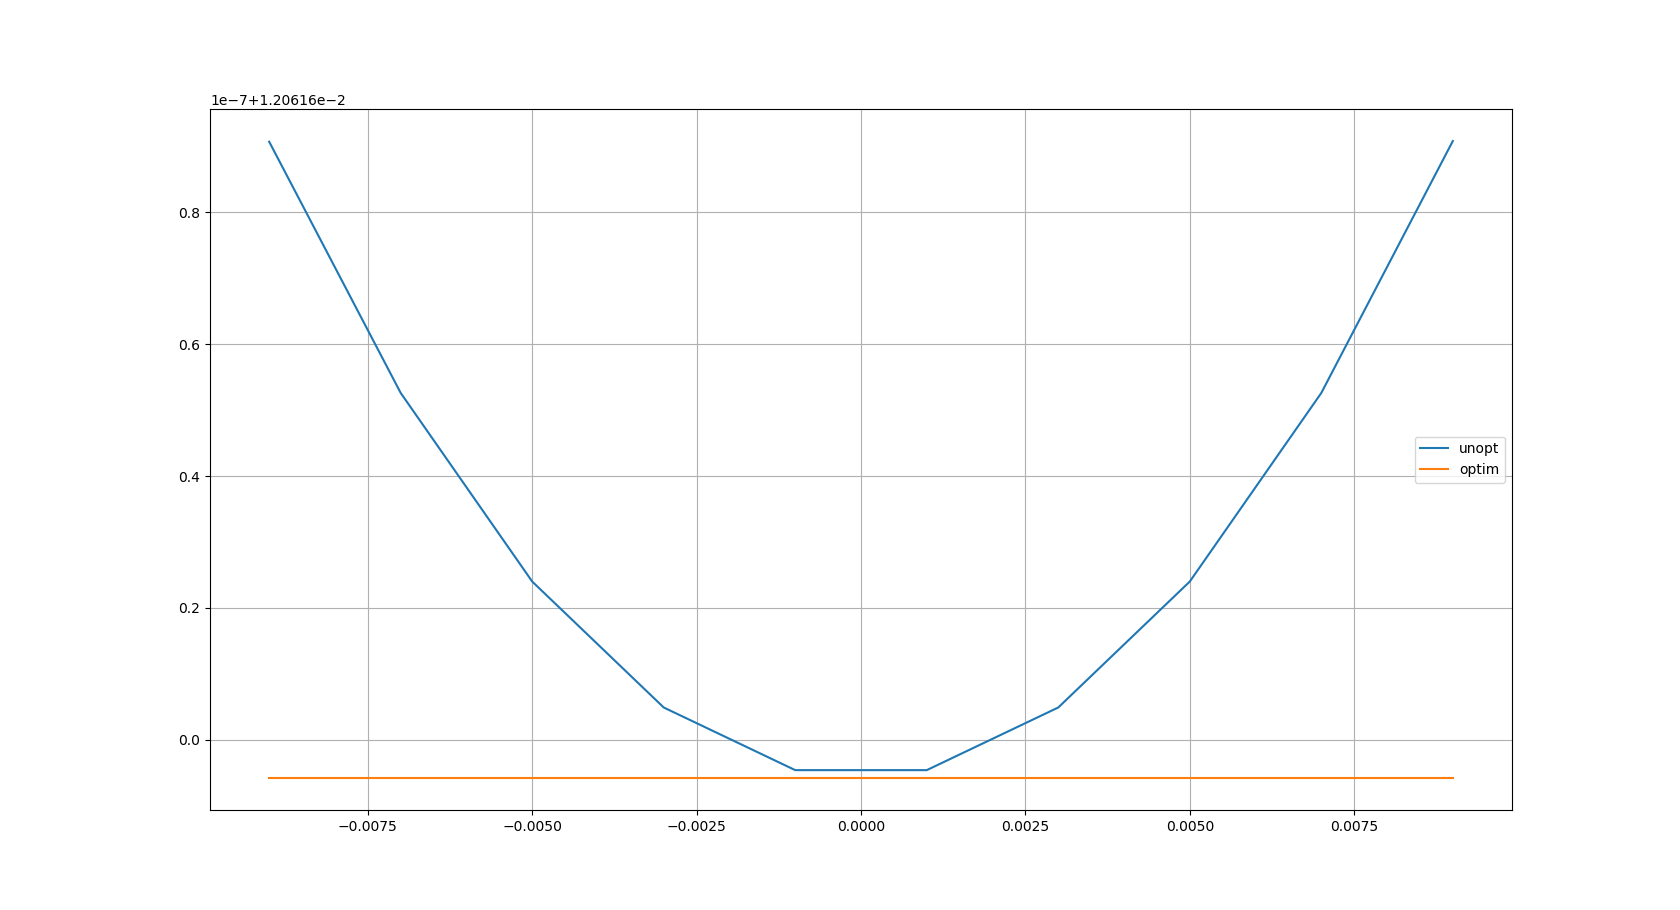
\includegraphics[width=\textwidth]{img/SPINTUNE_X_GSX_optim}
    \caption{GSX optimized for the X bunch}
  \end{subfigure}
  \begin{subfigure}[b]{\textwidth}\centering
    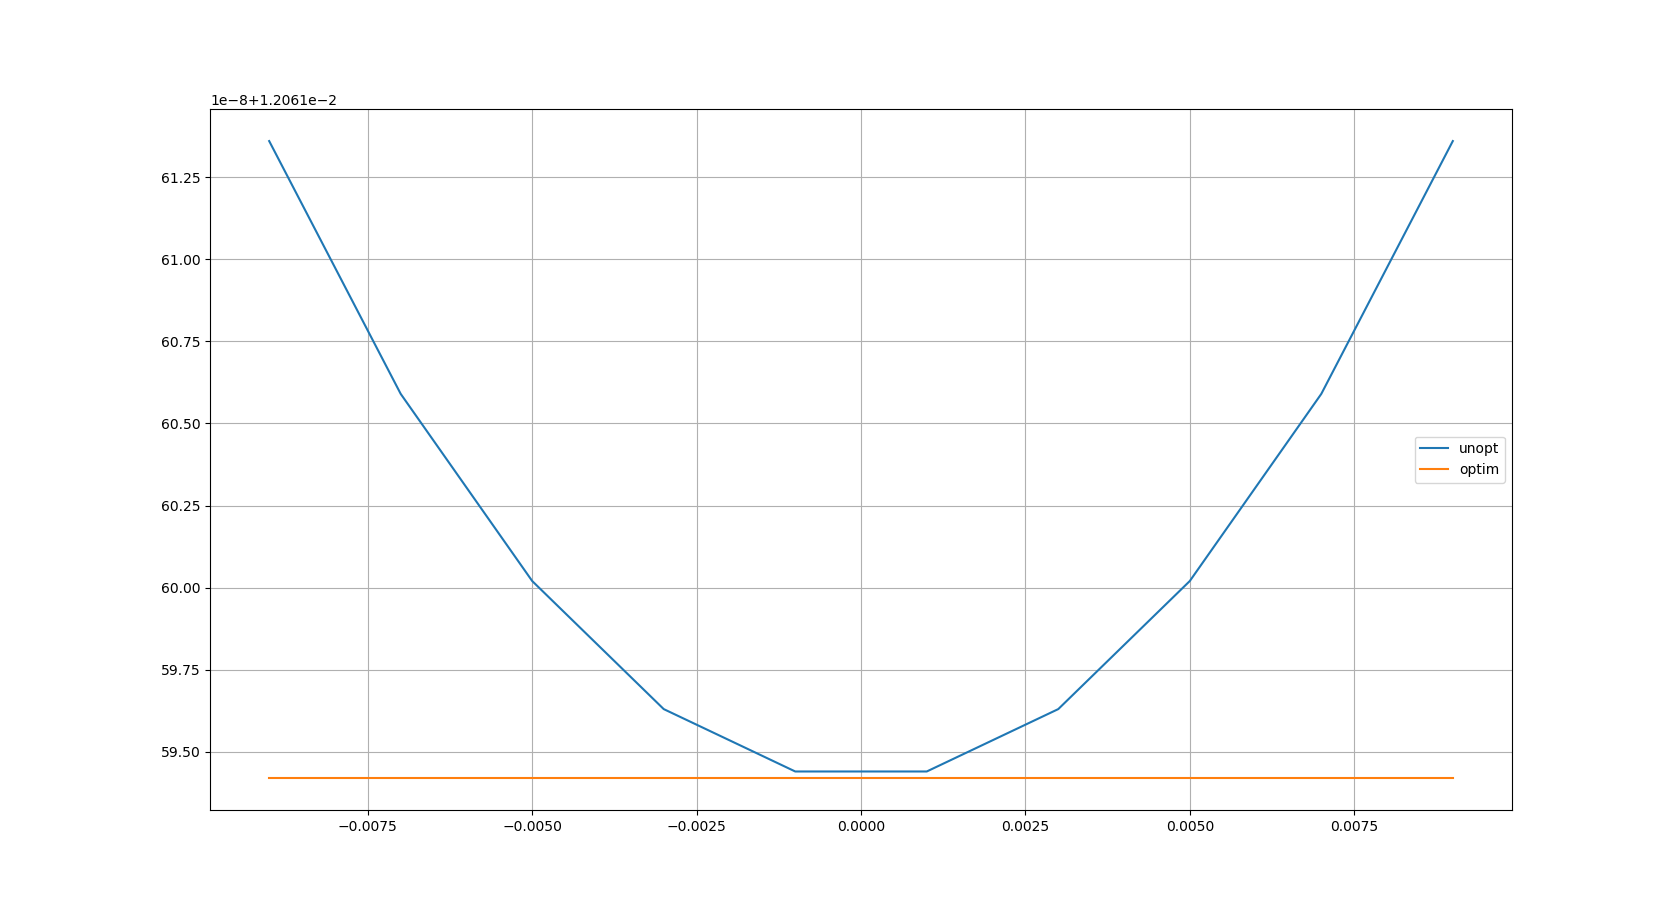
\includegraphics[width=\textwidth]{img/SPINTUNE_Y_GSY_optim}
    \caption{GSY optimized for the Y bunch}
  \end{subfigure}
\end{figure}
\begin{figure}\ContinuedFloat
  \begin{subfigure}[b]{\textwidth}\centering
    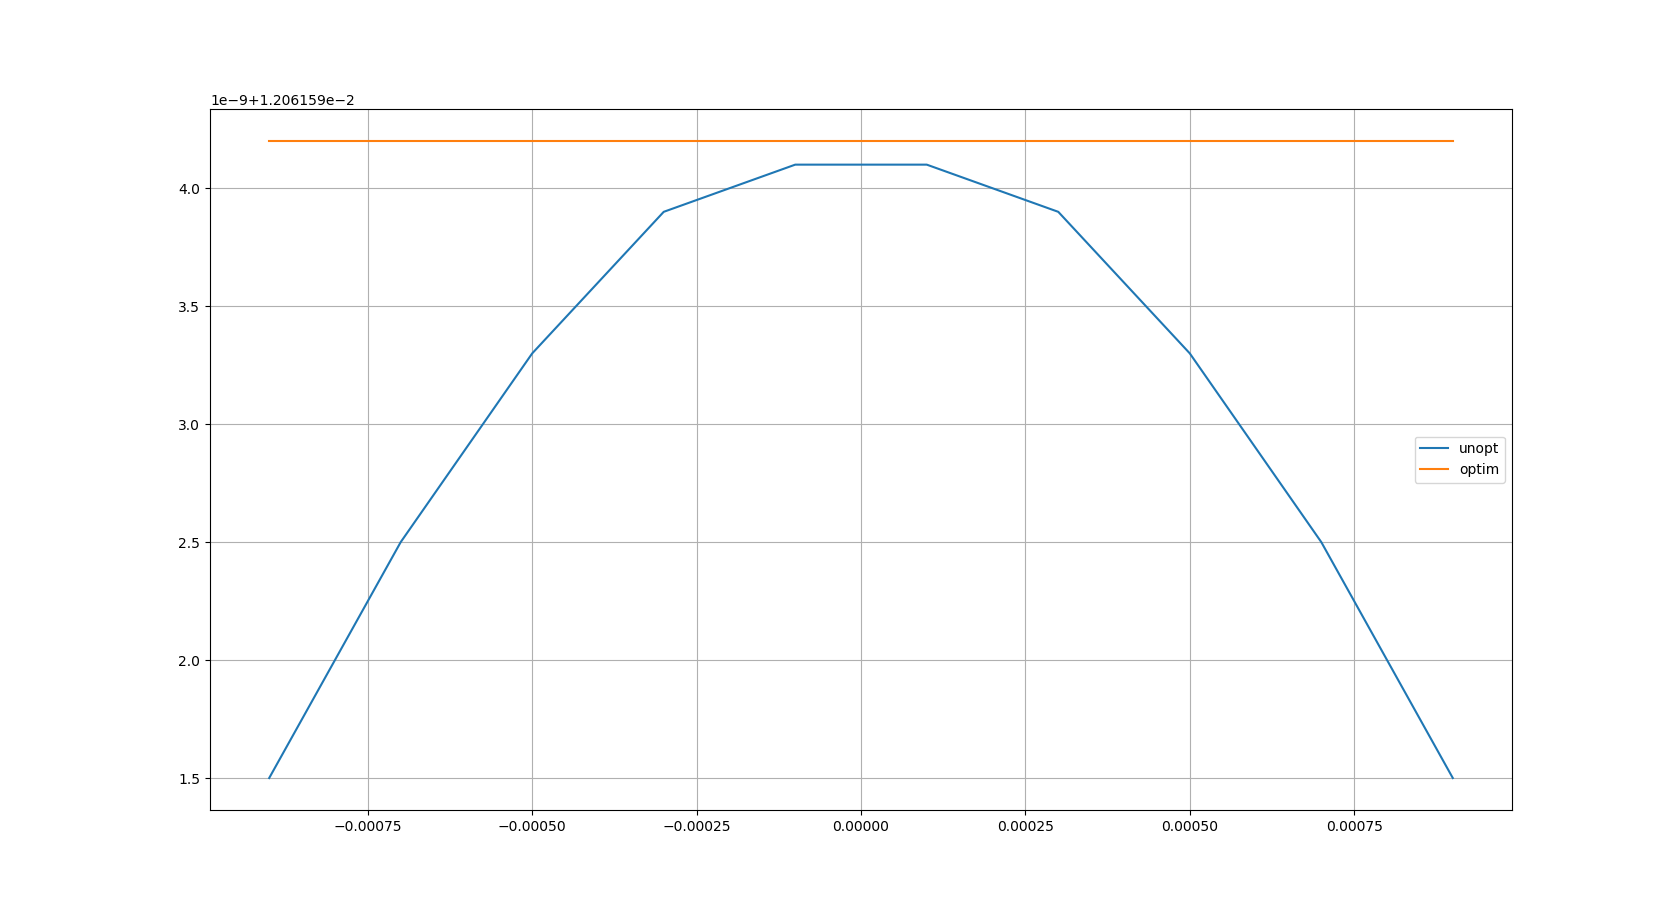
\includegraphics[width=\textwidth]{img/SPINTUNE_D_GSD_optim}
    \caption{GSD optimized for the D bunch}
  \end{subfigure}
  \caption{Spin tunes of offset particles vs the offsets, at 300 MeV, with/out the corresponding sextupole.\label{fig:OptSext}}
\end{figure}


\section{Fake signal simulation}

Systematic errors due to imperfections in the physical lattice, including optical element misalignments, are causative to a fake EDM signal.~\citep[p.~230]{Eremey:Thesis} Rotational misalignments are particularly problematic, since they induce the horizontal magnetic error field components $B_x$ and $B_z$ both of which rotate spin in the vertical plane, thus causing a fake EDM signal.

Analytical estimates of the MDM precession frequency about the radial axis were made by Senichev.~\cite{Senichev:FDM} From the T-BMT equation, and the expression for the Lorentz force, the MDM precession rate about the radial axis is
\begin{equation}
  \SD{\W_x^{MDM}} = \frac{q}{m\gamma}\frac{G+1}{\gamma}\frac{\SD{B_x}}{\sqrt{n}},
\end{equation}
where $n$ is the number of tilted spin rotators, and $\SD{B_x} = B_y \SD{\delta h}/L$, $\SD{\delta h}$  being the alignment error standard deviation. At alignment error $\SD{\delta h} = 100 \mu$m, and deflector length $L=1$m, $\SD{\W_x^{MDM}} \approx 100$ rad/sec.~\cite{Senichev:FDM}

We studied spin dynamics in the FS and QFS lattices in the presence of rotational magnet misalignments using the COSY INFINITY code. Our simulations appear to confirm the above analysis.

\subsection{Error field implementation}
In implementing field imperfections we followed the recommendations given in~\citep[p.~235]{Eremey:Thesis}. A small perturbation of the magnetic field acts with a first-order perturbation correction as a small proportional rotation on the spin vector. Therefore, we implemented rotational magnet misalignments as an augmentation of the rotated elements with small, normally-distributed spin kicks.

According to eq~\eqref{eq:TMBT_MDM}, the MDM precession frequency change associated with an introduced error field $(B_x, 0, B_z)$ is
\begin{align*}
  \Delta\W_{MDM} &= \frac qm (B_x, 0, B_z),
  \intertext{so the spin kick angle is}
  \Theta_{kick} &= t_0\Delta\W_{MDM},
\end{align*}
where $t_0 = L/v_0$ is the time-of-flight of the reference particle through the element.

\subsection{Simulation}
We randomly assigned tilt angles $\Theta_{tilt}$ to E+B elements in the FS lattice. The experiment was performed 11 times; each time the angles were selected from a normal distribution $N(\mu_0\cdot(i-5), \sigma_0)$, where $\mu_0 = 10\cdot \sigma_0 = 10^{-4}$ rad, $i\in\lbrace0,\dots, 10\rbrace$. After the construction of the 3rd order transfer map for the imperfect lattice, the spin tune and spin precession axis (SPA) Taylor expansions were computed. We then took the zero-order terms of the maps, representing the spin tune and SPA of the reference particle. The results are presented in Figure~\ref{fig:Linearity_test_shifting_gauss}. In Figure~\ref{fig:Linearity_test_compensated} are shown the results when three pairs of E+B elements are rotated by opposite angles, and one element is rotated by an angle $\mu_i = (i-5)\cdot 10^{-6}$ rad, $i\in\lbrace0,\dots,10\rbrace$. The simulations were done at 270.0092 MeV.\footnote{At this energy the spin precession axis and spin tune are undefined in the beamline coordinate system used by COSY INFINITY in the perfect lattice. This corresponds to the situation when spin does not precess in any plane (horizontal or vertical), which is the FS condition in a perfect lattice.}

\begin{figure}[h]
  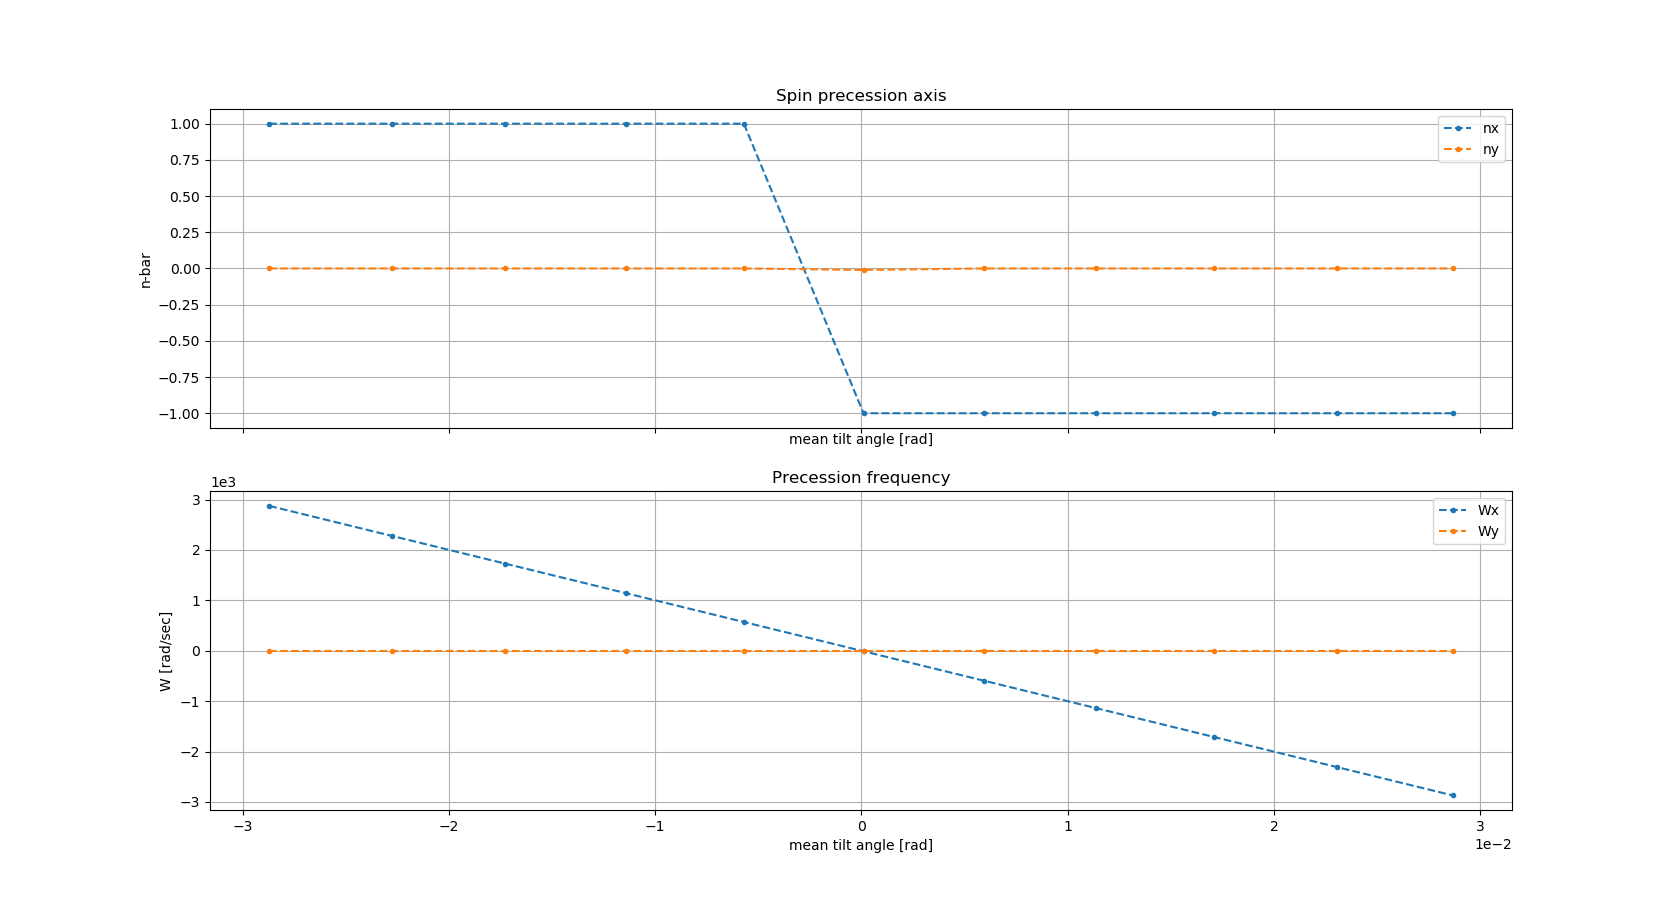
\includegraphics[width=\textwidth]{img/linearity_test_shifting_gauss}
  \caption{Spin precession axis and precession frequencies for the imperfect FS lattice, under the rotation of E+B elements.\label{fig:Linearity_test_shifting_gauss}}
\end{figure}
\begin{figure}[h]
  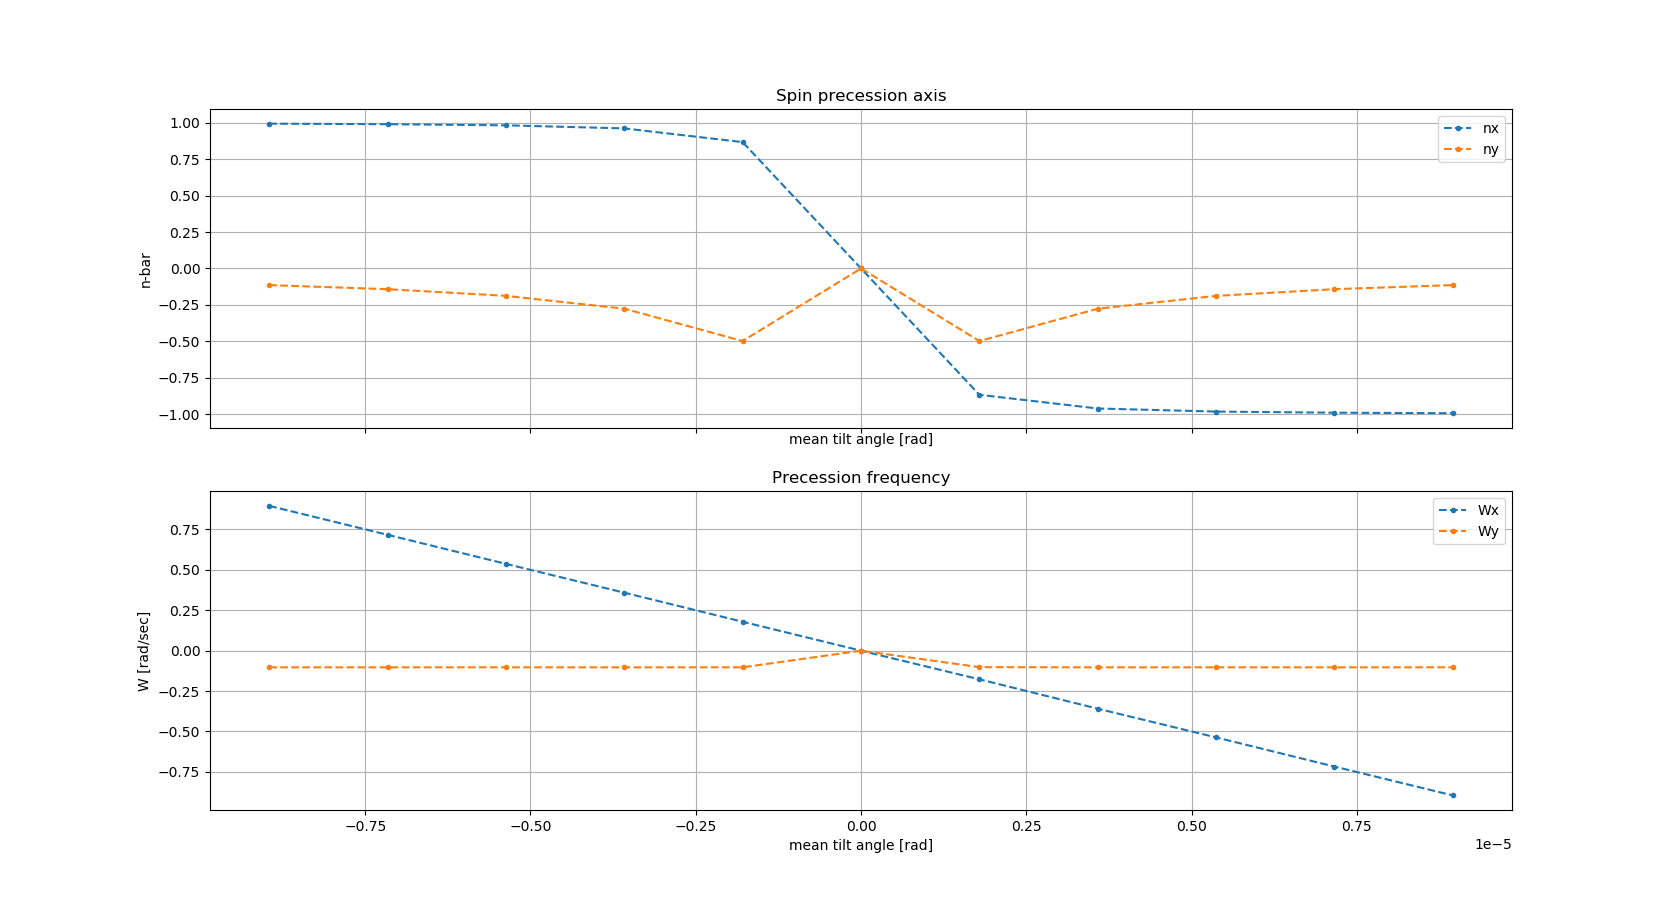
\includegraphics[width=\textwidth]{img/linearity_test_compensated+microrad}
  \caption{Three pairs of oppositely rotated E+B elements, plus an uncompensated element.\label{fig:Linearity_test_compensated}}
\end{figure}


\bibliography{PhDRefs}
\bibliographystyle{vancouver}

\end{document}
